\section{Experimental Results}\label{sec:results}

\mypar{Experimental setup} The improvements were evaluated on two different platforms:
\begin{itemize}
\item Intel\textsuperscript{\textregistered} Xeon CPU E3-1220L V2 @ 2.30 GHz, gcc (Debian 4.9.2-10) 4.9.2
\item Intel\textsuperscript{\textregistered} Core i5-2500 @ 3.3 GHz, Windows 8.1 using cygwin64 with gcc 4.9.2
\end{itemize}

\mypar{Baseline}
The analysis of the baseline implementation showed a lot of potential for optimization. Most notably by reducing memory overhead caused by object creation and deletion, random reads from lookup tables and vector operations. This can also be seen in the performance plot [ref to figure].

\mypar{Impact of Optimizations}
As can be seen in the runtime plot [ref to figure], the overall runtime was reduced by a factor of 7 to 25 depending on input size. Most of these improvements were achieved by reducing the number of operations by a factor of x as shown in figure [ref to figure]. One particular optimization (build 6) replaced many multiplications with one division. Due to such optimizations the performance of the optimized version did not improve, as shown by the roofline analysis \cite{Ofenbeck:14} shown in figure \ref{roofline-mixed}.

\begin{figure}\centering
    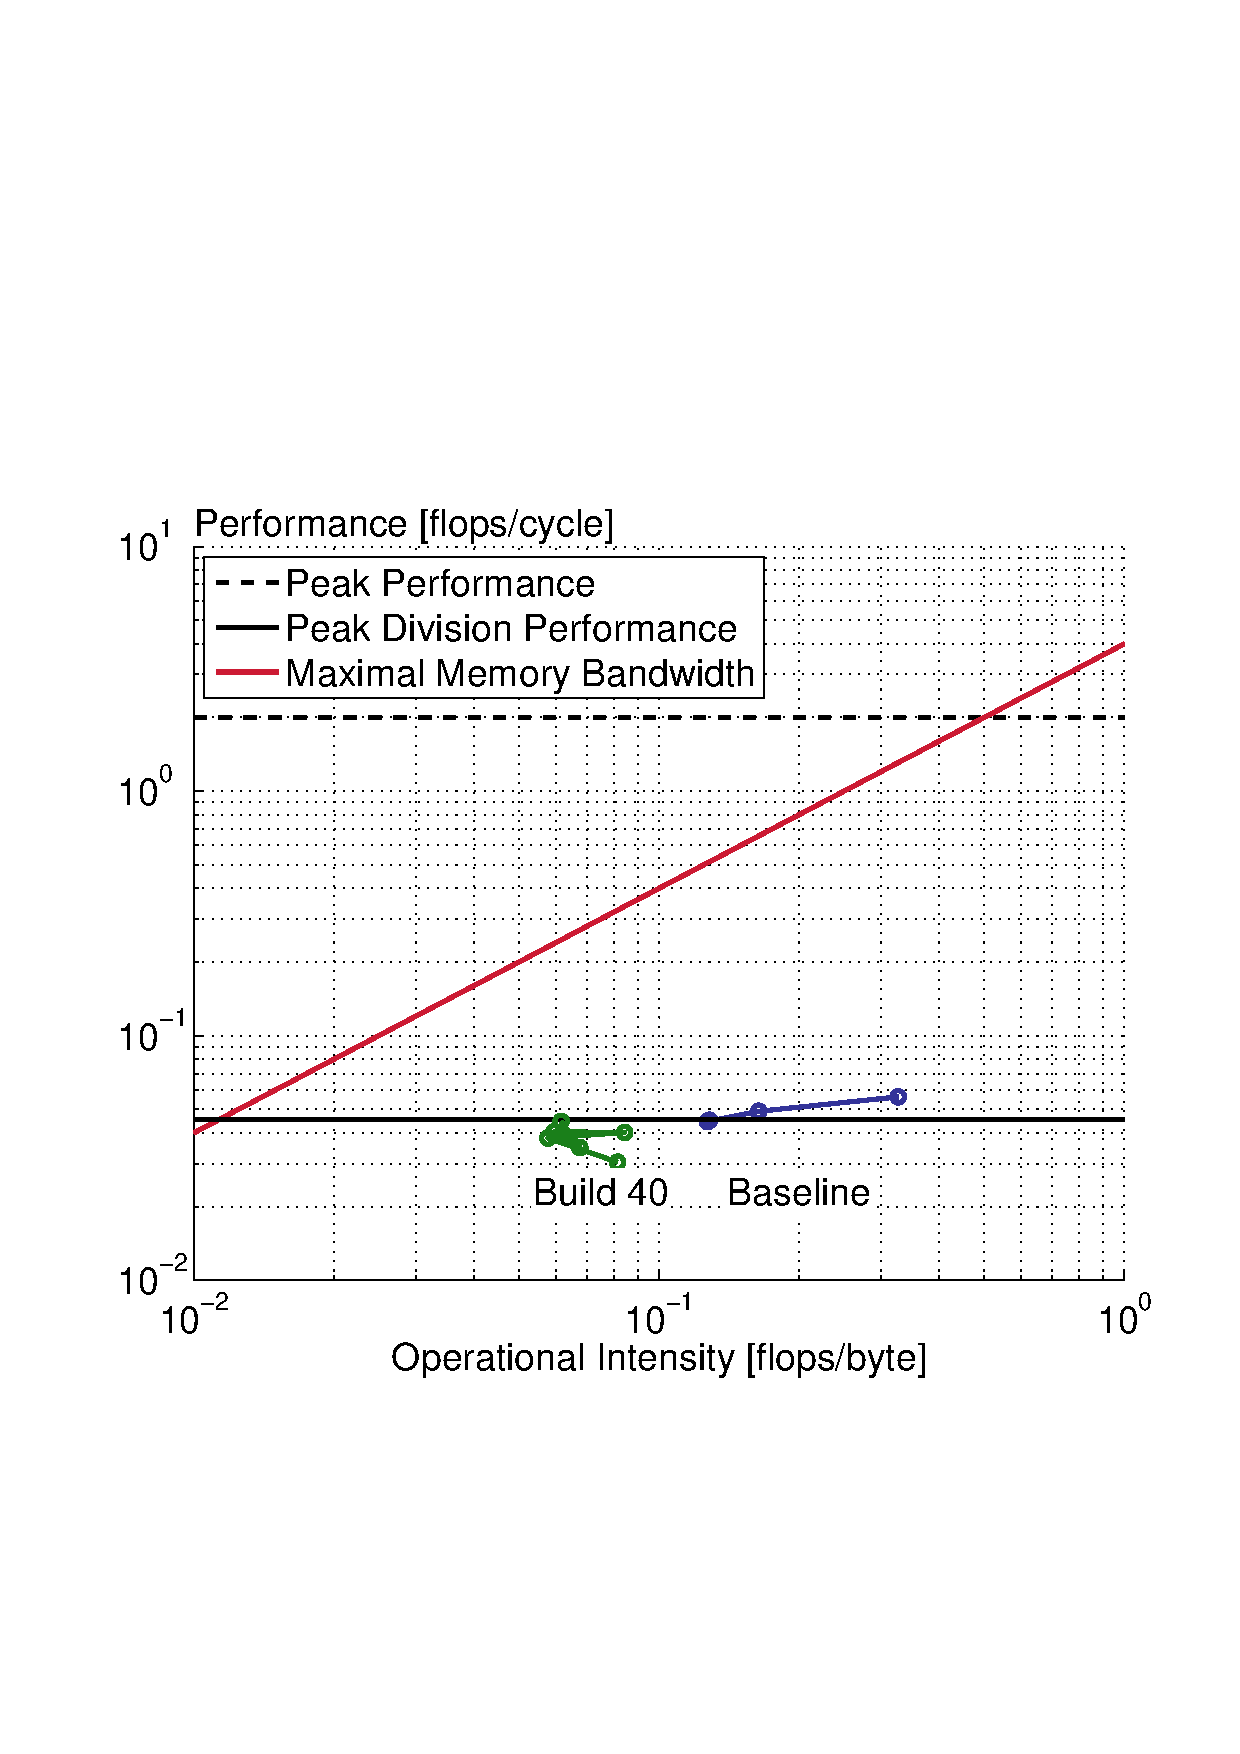
\includegraphics[scale=0.48, trim={2cm 6.5cm 1cm 8.5cm},clip]{graphics/roofline_mixed.pdf}
  \caption{Roofline analysis of the baseline and our optimized version (build 40). The analysis was conducted on the Windows system described above.\label{roofline-mixed}}
\end{figure}

\begin{figure*}\centering
  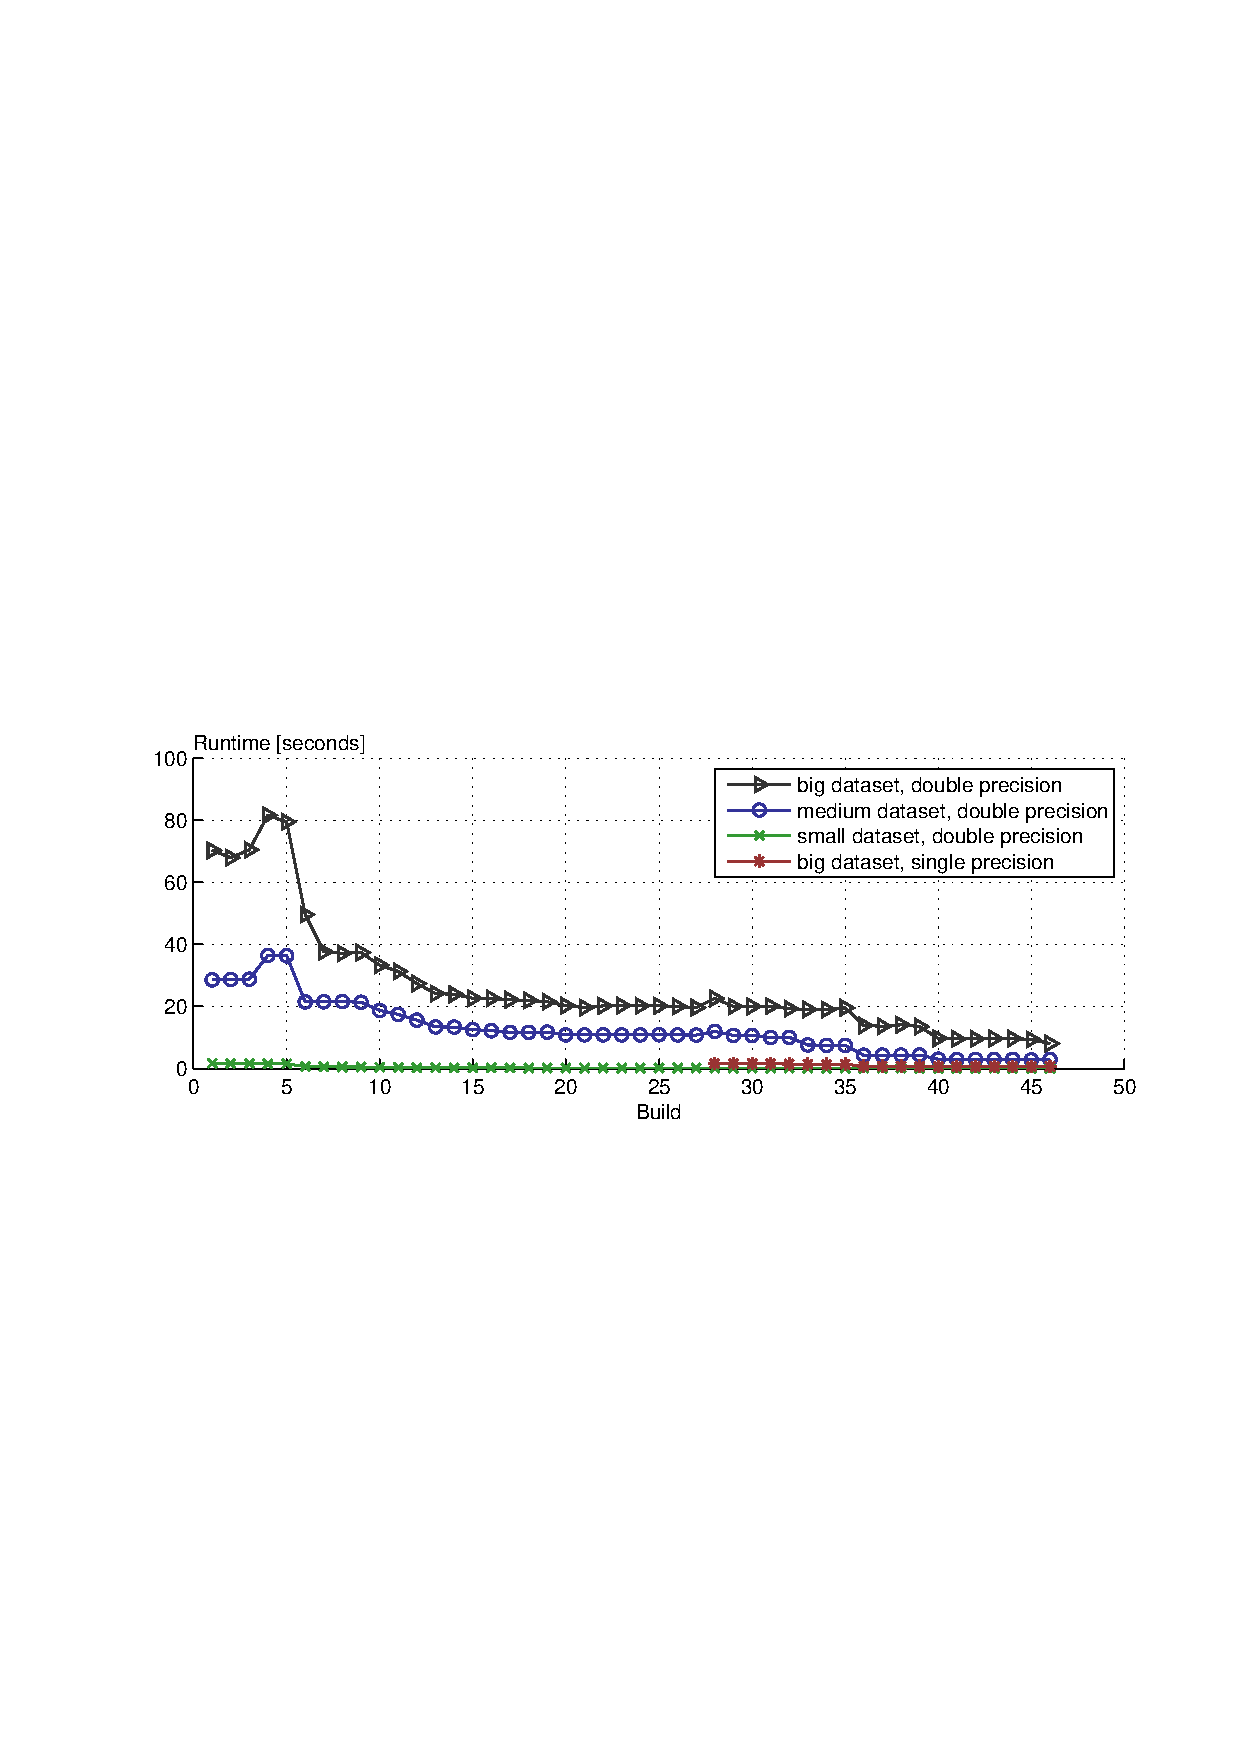
\includegraphics[scale = 1, trim={6cm 11cm 5cm 14cm}]{graphics/runtime_plot.pdf}
  \caption{This is a tiger.}
\end{figure*}

\mypar{Vectorization}
To further improve the runtime some parts of the code were vectorized manually. Unfortunately, this did not bring a significant improvement.

